\documentclass{article}

	\usepackage[margin=1in]{geometry}
	
	\usepackage[backend=bibtex, style=authoryear]{biblatex}
		
	\addbibresource{sources/sources.bib}
	\usepackage{hyperref}
	
			\title{\textsc{Data Inversion Using Neural Networks for Computed Tomography Imaging Spectrographs}}
			\date{\today}
			\author{Roy Smart \\ \url{roy.smart@montana.edu} \\ Montana State University, Department of Physics \\ Bozeman, MT 59717, USA}
			
	\usepackage{float}
	\usepackage{graphicx}


\begin{document}

	\maketitle
	
	\tableofcontents
	
	\begin{abstract}
		
	\end{abstract}
		
	
	\section{Problem Statement}
		\subsection{Background}
		
			Spectrometers are important tools for solar astronomy. This is due to the fact that the Sun has a complex spectral structure, composing of numerous emission and absorption lines exhibiting variations in linewidth, mean wavelength and intensity. Many spectrographic structures such as explosive events, first described by (\cite{dere1}), have yet to be fully explained, indicating that there is still much to be learned concerning the spectral structure of the sun.
			
			Conventional spectrographs such as \textit{IRIS}, split light into its component spectra using a diffraction grating and then use a slit to restrict the spatial field of view along the dispersion direction of the diffraction grating (\cite{De Pontieu2014}). This configuration yields images that represent the intensity of the light source as a 1D function of space (perpendicular to the dispersion direction) and a 1D function of wavelength. To acquire intensity information along the dispersion direction, conventional spectrographs are often operated in raster mode, where the slit is scanned parallel to the dispersion direction. This process builds up a \textit{spatial-spectral cube}, which contains the intensity of the light source as a 2D function of space and a 1D function of wavelength. Unfortunately the cube acquired through the process of rastering is not cotemporal, \textit{i.e.} each of the images within the cube was taken at a different time, governed by the readout speed of the imager and the scanning speed of the slit. 		
		
			Computed tomography imaging spectrographs (CTISs) are a relatively new type of instrument that has been independently developed by multiple parties including: \cite{Okamoto:91}, \cite{bulygin:92}, \cite{Descour:95}, and \cite{kankel1}. This type of instrument promises to recover a cotemporal, spatial-spectral cube. CTISs accomplish this using a diffraction grating, similar to those used by conventional spectrographs, but unlike conventional spectrographs, CTISs are not equipped with a slit, allowing them to observe a wide field of view in both spatial directions. Without the slit, the spectral and spatial information from the light source is convolved into a single image. Since this convolution operation is not easily inverted, images are formed in multiple diffraction orders to provide enough information to reconstruct the spatial-spectral cube (\cite{inversion}).	
			 
		\subsection{Inversion}
		
			Computing the spatial spectral cube using images formed at multiple diffraction orders can be interpreted as a classic 3D tomography problem where $N$ projections are taken through a translucent 3D object in $x$, $y$ and $\lambda$ space (\cite{Bulygin:05}).
			\begin{figure}[h!]
				\centering
				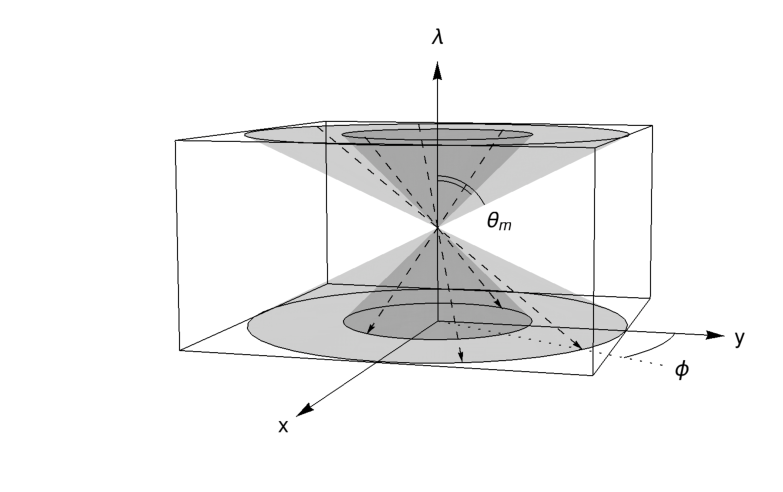
\includegraphics[width=0.5\textwidth]{figures/tomography}
				\caption{Geometry of the inversion problem for CTIS interpreted as a 3D tomography problem. $\theta_i$ represents the diffraction order and takes on discrete values, while $\phi$ represents the dispersion direction. Figure taken from \cite{Bulygin:05}}
				\label{tomography}
			\end{figure}
			In this interpretation, the usual polar angle $\theta$ represents the diffraction order ($i=0,1,2,3,...$) and therefore takes discrete values. Note that $\theta=0$ corresponds to the $i=0$ order, which is equivalent to an image that would be produced by a telescope, for example.
			
			Using this representation, we can write the intensity of an object $v(x,y,\lambda)$ viewed by a CTIS in terms of the intergral equation provided by \cite{fox1}
			\begin{equation}
				I_i (x',y') = \int_B v(x' - \lambda \tan \theta_i \cos \phi, y' - \lambda \tan \theta_i \sin \phi, \lambda) \; d\lambda,
				\label{tomo_eqn}
			\end{equation}
			where $x'$ and $y'$ are image coordinates and $B$ is the passband of the instrument. Equation \ref{tomo_eqn} is a Fredholm integral equation of the first kind (\cite{RHB}) with a projection kernel. Our goal is then to invert Equation \ref{tomo_eqn} to recover the object $v(x,y,\lambda)$.
			
			The CTISs developed by Charles Kankelborg and his research group only take between $N=3$ and $N=6$ projections through the spatial-spectral cube. This limited number of projections does not provide enough information to completely reconstruct the spatial-spectral cube, \textit{i.e.} in the case of the CTISs discussed below (MOSES and ESIS), inverting Equation \ref{tomo_eqn} is an ill-posed problem (\cite{inversion}). We can see this by noting that for a spatial spectral cube of length $L$ in both spatial directions, and a depth $M$ in the spectral direction the amount of information in the cube is $I_c = L^2 \times M$ and the the information provided by all the projections is $I_p = L^2 \times N$. So therefore to build a spatial-spectral cube of appreciable resolution, an inversion algorithm will need to use physical constraints to gain enough information to reconstruct the spatial-spectral cube. In Section \ref{pwork} we will briefly explore advantages and disadvantages of the physical constraints used by current inversion algorithms, and in Section \ref{prop_sol} we will propose to use machine learning algorithms to construct these physical constraints and solve the inversion problem.
			
		\subsection{Current and Planned CTISs}

			In the sections below, we will conduct a limited overview of the current and planned CTISs designed and build by Charles Kankelborg and his research group. A brief understanding of the optical system of each instrument will be helpful to understanding the goals of this proposal. 

			Each of the instuments in the succeeding sections is designed to fly on a Black Brant IX sounding rocket launched from White Sands Missile Range. Additionally, each instrument is constructed with a narrow passband in EUV. This narrow passband aims to alleviate the inherit diffuculty in the inversion process.

			\subsubsection{MOSES I}



			\subsubsection{MOSES II}
			\subsubsection{ESIS}
		\subsection{Previous Work}
			\label{pwork}
		\subsection{Project Goals}
	\section{Proposed Solution}
		\label{prop_sol}
		\subsection{Introduction to Neural Networks}
		\subsection{Inversion Using Neural Networks}
	\section{Relevance to Heliophysics}
	\section{Project Timeline}
	

	\printbibliography

	
\end{document}

